\chapter{Arquitectura de la Solución}

Este capítulo describe la arquitectura técnica del MVP ContractIA: las capas
que lo componen, el pipeline de procesamiento, las decisiones de diseño
adoptadas y el stack tecnológico seleccionado. La arquitectura fue diseñada
para ser funcional y desplegable en producción desde el primer día, priorizando
la simplicidad operable sobre la optimización prematura.

% ─────────────────────────────────────────────────────────────────────────────
\section{Visión General}

ContractIA implementa una arquitectura en capas desplegada íntegramente en
Google Cloud Platform (GCP), con un núcleo de procesamiento multi-agente y
dos interfaces de acceso para el usuario final. La arquitectura se organiza
en cuatro capas principales:

\begin{enumerate}
    \item \textbf{Capa de Interfaz:} Bot Telegram y frontend web (Next.js)
    como puntos de entrada para el usuario.
    \item \textbf{Capa de Backend:} API REST (FastAPI) como hub central que
    orquesta el pipeline de análisis, gestiona la cola de trabajos y expone
    los resultados.
    \item \textbf{Capa de Inteligencia:} Motor multi-agente (Jurista, Auditor,
    Cronista) con RAG híbrido (FAISS + BM25 + Cohere) y GraphRAG, consumiendo
    Gemini~2.5~Pro vía Vertex~AI.
    \item \textbf{Capa de Datos:} PostgreSQL~15 (Cloud SQL) para persistencia
    de auditorías y usuarios, y Google Cloud Storage para contratos y reportes.
\end{enumerate}

\begin{figure}[H]
    \centering
    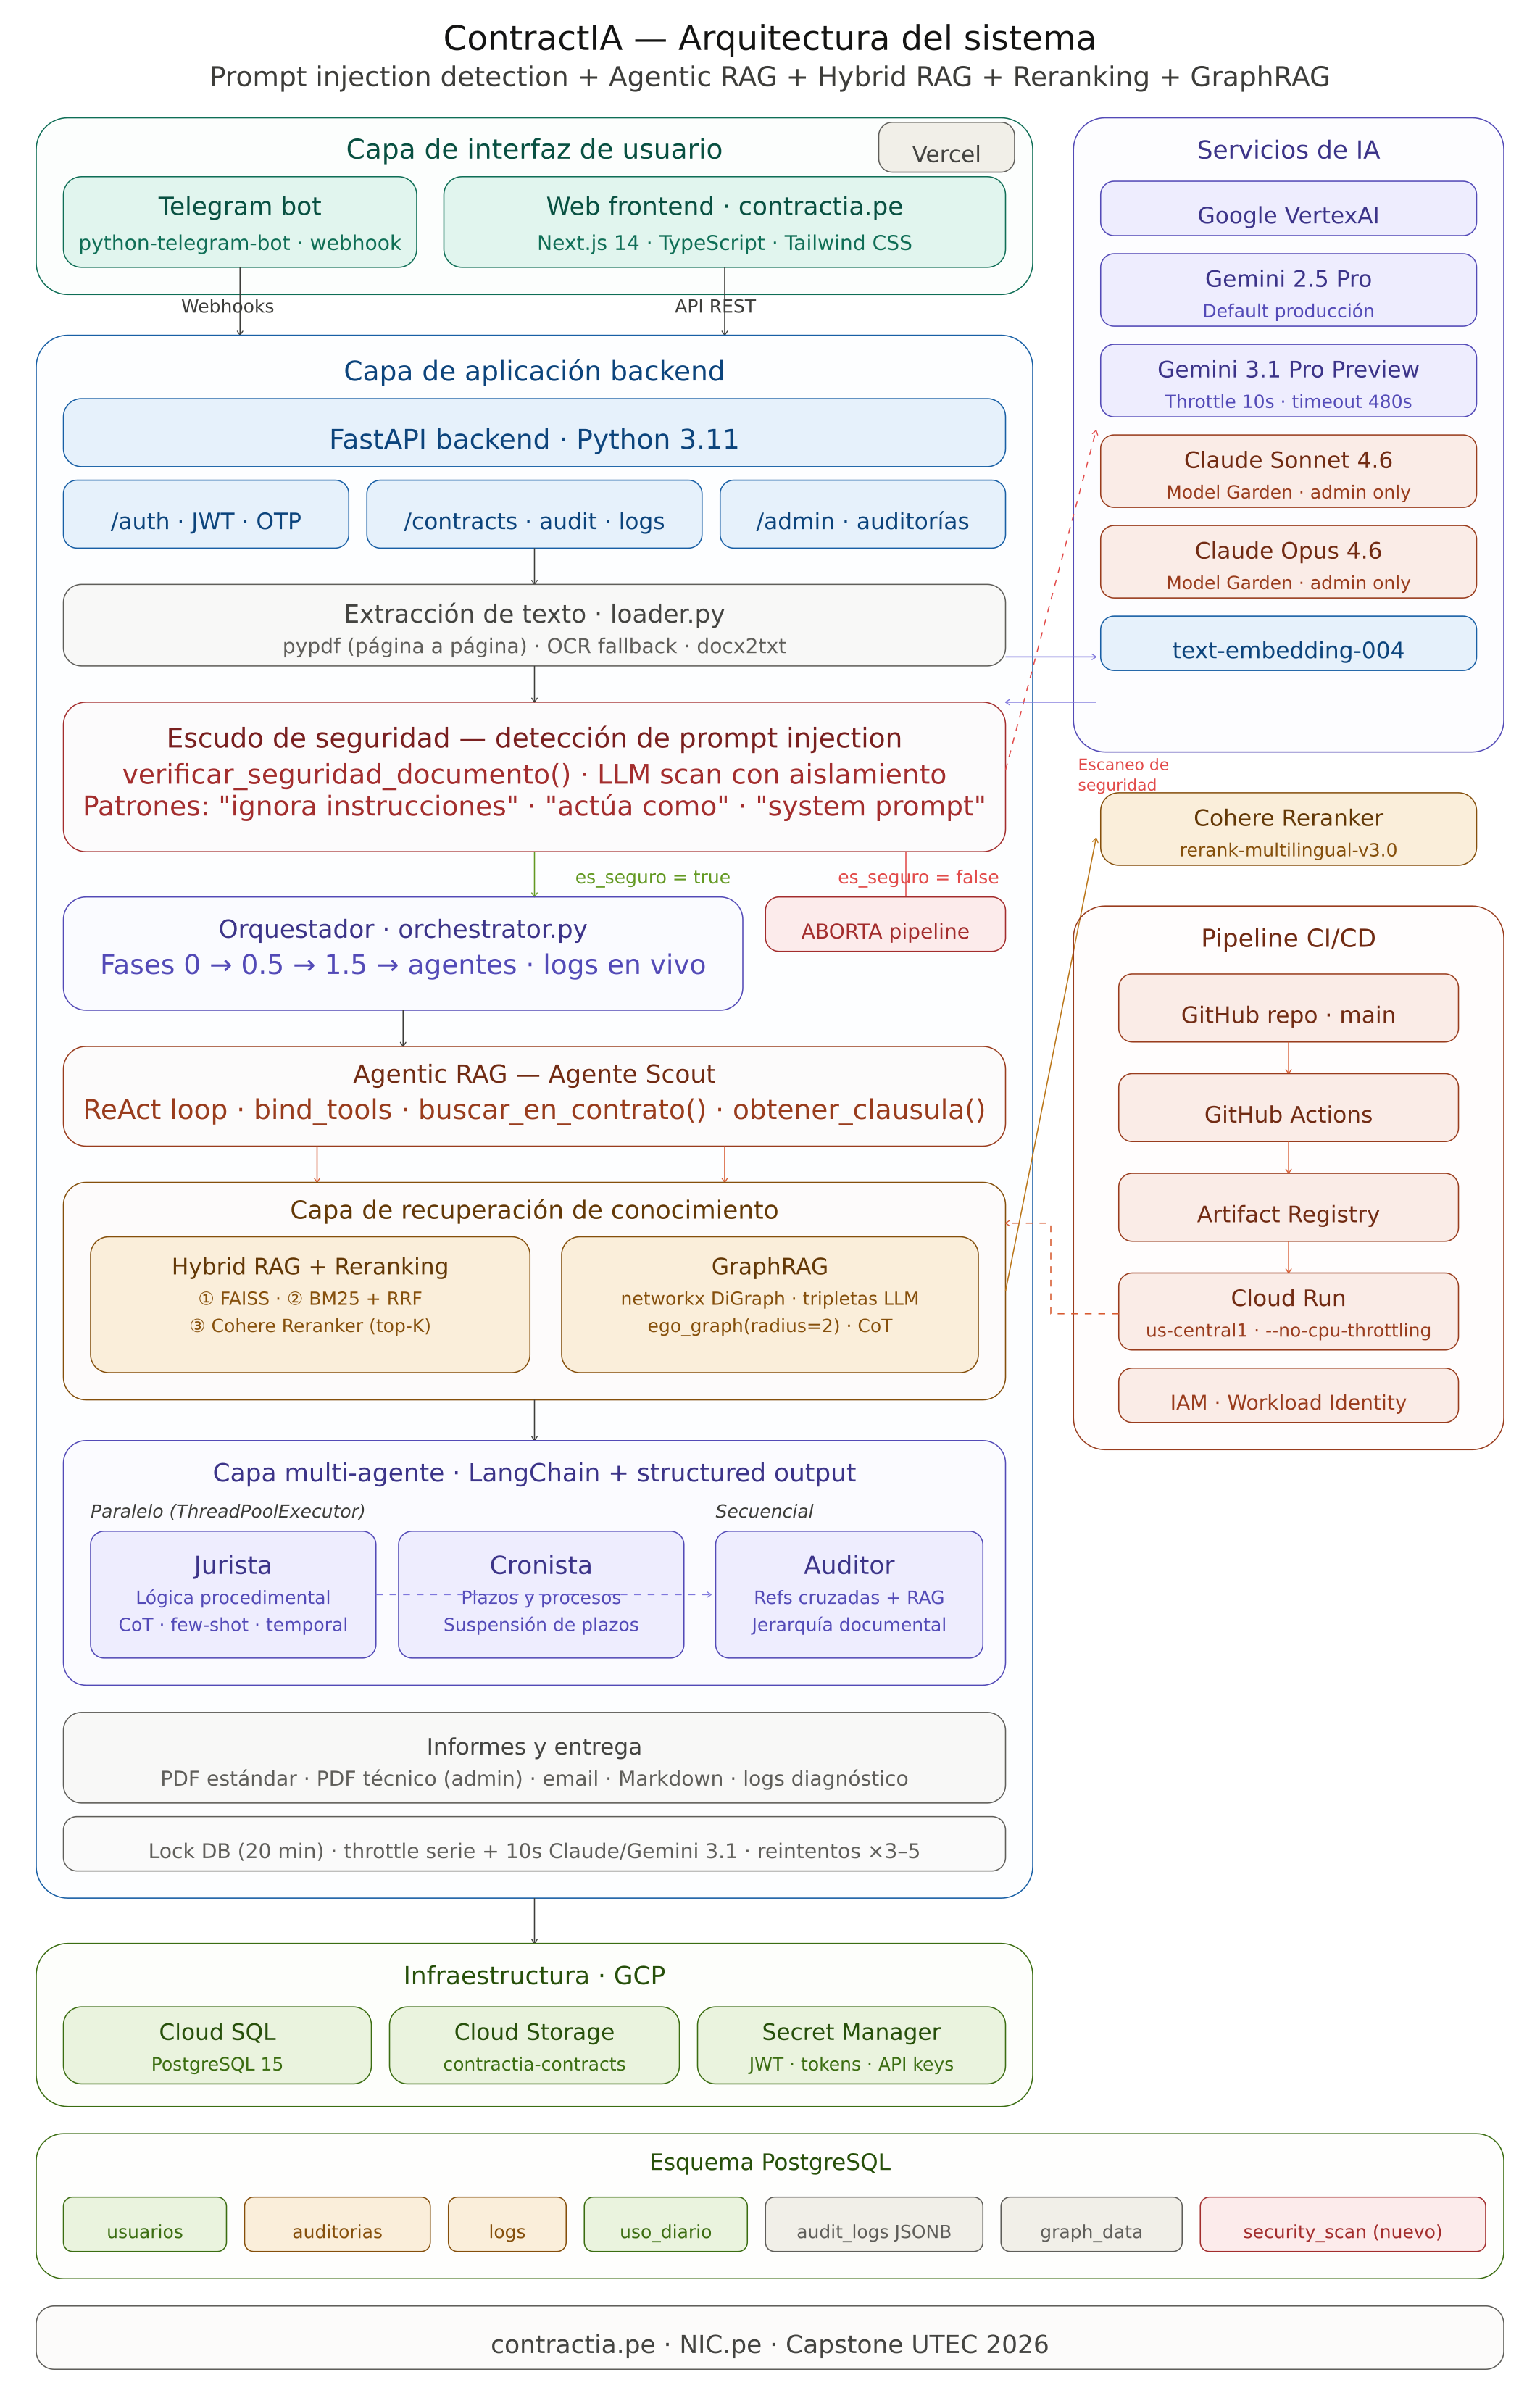
\includegraphics[width=0.87\linewidth]{images/contractia_architecture_centered.png}
    \caption{Arquitectura Detallada}
    \label{fig:Arquitectura Detallada}
\end{figure}

% ─────────────────────────────────────────────────────────────────────────────
\section{Flujo de Procesamiento End-to-End}

El pipeline de auditoría sigue un flujo secuencial de fases bien definidas,
ejecutadas de forma autónoma tras la carga del contrato:

\begin{table}[H]
\centering
\caption{Fases del pipeline de auditoría ContractIA}
\label{tab:pipeline}
\begin{tabular}{p{0.5cm} p{3.5cm} p{4.5cm} p{5cm}}
\toprule
\textbf{\#} & \textbf{Fase} & \textbf{Componente} & \textbf{Resultado} \\
\midrule
0 & Segmentación & Regex + Anti-TOC & 41 secciones (contrato piloto) \\[3pt]
0.5 & Indexación multinivel & FAISS + índice global & 448 cláusulas indexadas \\[3pt]
1 & RAG híbrido & FAISS + BM25 + Cohere & Contexto normativo por sección \\[3pt]
1.5 & GraphRAG & NetworkX DiGraph + LLM & Grafo de relaciones contractuales \\[3pt]
2 & Análisis multi-agente & Jurista + Auditor + Cronista & Hallazgos trazados por sección \\[3pt]
3 & Consolidación & Orquestador + Pydantic & Reporte JSON estructurado \\[3pt]
4 & Generación de reporte & FastAPI + Cloud Storage & PDF ejecutivo descargable \\[3pt]
5 & Notificación & Email automático & Aviso al usuario al finalizar \\
\bottomrule
\end{tabular}
\end{table}

% ─────────────────────────────────────────────────────────────────────────────
\section{Capa de Ingesta}

El sistema recibe contratos a través de dos canales: la API REST (carga
directa vía frontend web) y el bot Telegram (carga conversacional). El
proceso de ingesta comprende:

\begin{itemize}
    \item \textbf{Extracción de texto:} PyMuPDF como extractor principal,
    con \textit{pdfminer} como fallback para PDFs con estructura compleja.
    Normalización UTF-8 y detección de páginas ilegibles o con OCR defectuoso.
    \item \textbf{Almacenamiento:} El contrato se persiste en Google Cloud
    Storage con un identificador único de auditoría. El registro de la
    auditoría se crea en PostgreSQL con estado \texttt{pendiente}.
    \item \textbf{Cola de trabajos:} Cada usuario puede tener hasta 5 trabajos
    pendientes. El sistema procesa un contrato activo a la vez por usuario;
    los demás quedan en cola y se procesan secuencialmente.
\end{itemize}

% ─────────────────────────────────────────────────────────────────────────────
\section{Pipeline de Procesamiento Estructural}

\subsection{FASE 0 — Segmentación automática}

El segmentador identifica capítulos y anexos mediante expresiones regulares
calibradas para contratos de concesión peruanos. Incluye:

\begin{itemize}
    \item \textbf{Mecanismo anti-TOC:} Filtra títulos duplicados originados
    en las tablas de contenido del documento, evitando secciones fantasma
    con cero cláusulas.
    \item \textbf{Resolución por densidad:} Cuando dos secciones compiten
    por el mismo título, prevalece la de mayor densidad de cláusulas.
    \item \textbf{Resultado en contrato piloto:} 20 capítulos + 21 anexos
    = 41 secciones con cobertura del 100\%.
\end{itemize}

\subsection{FASE 0.5 — Indexación multinivel}

Se construyen tres índices complementarios para soportar el análisis:

\begin{itemize}
    \item \textbf{Índice Global de Cláusulas:} Mapeo de todas las cláusulas
    del contrato con su número, sección y texto. El contrato piloto produjo
    448 entradas.
    \item \textbf{Índice de Secciones:} Metadatos de cada sección (título,
    rango de páginas, número de cláusulas).
    \item \textbf{Índice Local por sección:} Permite búsqueda de cláusulas
    dentro del contexto de una sección específica durante el análisis.
\end{itemize}

\subsection{FASE 1 — RAG Híbrido}

El módulo RAG combina tres estrategias de recuperación para maximizar la
relevancia del contexto normativo:

\begin{itemize}
    \item \textbf{FAISS (semántico):} Vectorización con
    \texttt{text-embedding-004} (Vertex~AI, 768 dimensiones). Recuperación
    por similitud coseno sobre la base normativa vectorizada (Ley de APP,
    TUO de Contrataciones, normas OSITRAN, OSINERGMIN, SUNASS).
    \item \textbf{BM25 (léxico):} Captura coincidencias exactas de términos
    legales, números de artículo y denominaciones específicas que los
    embeddings semánticos pueden subestimar.
    \item \textbf{Cohere Rerank v3:} Reordena los fragmentos recuperados por
    ambos métodos según su relevancia contextual real, reduciendo el ruido
    en el contexto enviado al LLM.
\end{itemize}

\subsection{FASE 1.5 — GraphRAG}

El módulo GraphRAG enriquece el análisis con contexto relacional:

\begin{itemize}
    \item \textbf{Extracción de tripletas:} El LLM extrae relaciones del tipo
    (origen, tipo\_relación, destino) por sección. Tipos de relación:
    \texttt{REFERENCIA\_A}, \texttt{ESTABLECE\_PLAZO}, \texttt{MODIFICA\_A},
    \texttt{DEPENDE\_DE}, \texttt{OBLIGA\_A}.
    \item \textbf{Grafo DiGraph (NetworkX):} El contrato piloto generó entre
    208 y 477 nodos y entre 258 y 617 relaciones, según el modelo empleado.
    \item \textbf{Uso en auditoría:} El orquestador consulta el grafo para
    identificar qué otras secciones tienen relaciones con la sección bajo
    análisis, enriqueciendo el contexto de cada agente.
\end{itemize}

% ─────────────────────────────────────────────────────────────────────────────
\section{Motor Multi-Agente (FASE 2)}

El núcleo analítico de ContractIA son tres agentes especializados que operan
en paralelo sobre cada sección del contrato:

\begin{table}[H]
\centering
\caption{Agentes especializados del motor de auditoría}
\label{tab:agentes}
\begin{tabular}{p{2.5cm} p{5cm} p{6cm}}
\toprule
\textbf{Agente} & \textbf{Especialización} & \textbf{Tipos de hallazgo} \\
\midrule
\textbf{Jurista} &
  Coherencia legal y semántica entre cláusulas &
  Contradicciones entre obligaciones, referencias semánticas incorrectas,
  ambigüedades en definiciones, omisiones normativas \\[4pt]
\textbf{Auditor} &
  Validación estructural y referencias cruzadas &
  Referencias a cláusulas inexistentes, numeración inconsistente,
  definiciones no utilizadas, secciones huérfanas \\[4pt]
\textbf{Cronista} &
  Coherencia temporal y de plazos &
  Plazos contradictorios, secuencias de hitos imposibles,
  inconsistencias en fechas de vigencia \\
\bottomrule
\end{tabular}
\end{table}

El \textbf{Orquestador} coordina la ejecución de los tres agentes mediante
\texttt{asyncio.gather}, consolida sus hallazgos eliminando duplicados y
aplica clasificación de severidad automática (ALTA / MEDIA / BAJA).
Los agentes utilizan \texttt{with\_structured\_output} de LangChain~0.3+
con esquemas Pydantic para garantizar salida JSON reproducible y tipada.

Para modelos LLM con cuota restringida (Claude~Sonnet, Gemini~3.1~Pro
Preview), el sistema aplica ejecución en serie con pausa de 30~s entre
llamadas para evitar errores 429.

% ─────────────────────────────────────────────────────────────────────────────
\section{Capa de Servicios e Infraestructura}

\begin{itemize}
    \item \textbf{API REST (FastAPI + Python~3.11):} Hub central con
    endpoints para carga de contratos, inicio y seguimiento de auditorías,
    consulta de estado por polling, descarga de reportes y administración
    de usuarios. Autenticación JWT con cuatro roles:
    \texttt{pendiente / básico / auditor / admin}.
    \item \textbf{Google Cloud Run:} Servicio containerizado con auto-scaling
    y disponibilidad $\geq 99\%$. Imagen Docker almacenada en Artifact
    Registry; despliegue continuo vía GitHub Actions con Workload Identity
    Federation (sin credenciales estáticas).
    \item \textbf{Cloud SQL (PostgreSQL~15):} Persistencia de auditorías,
    hallazgos individuales, logs de procesamiento y gestión de usuarios.
    Conexión segura vía Cloud SQL Auth Proxy.
    \item \textbf{Google Cloud Storage:} Almacenamiento de contratos PDF/DOCX
    cargados y reportes ejecutivos generados, con URLs firmadas de descarga.
    \item \textbf{Secret Manager:} Gestión centralizada de credenciales
    (API keys de Vertex~AI, Cohere, JWT secret) sin exposición en código
    ni variables de entorno en texto plano.
\end{itemize}

% ─────────────────────────────────────────────────────────────────────────────
\section{Interfaces de Usuario}

\begin{itemize}
    \item \textbf{Frontend web (Next.js~14, TypeScript, Tailwind CSS):}
    Dashboard de auditorías con panel de diagnóstico técnico en tiempo real
    (polling SSE), visualización de hallazgos por severidad, descarga de
    reportes PDF. Desplegado en \texttt{contractia.pe} vía Vercel.
    \item \textbf{Bot Telegram (python-telegram-bot~20+):} Interfaz
    conversacional para carga de contratos, seguimiento de progreso en cola,
    descarga de reportes y gestión de accesos (aprobación de nuevos usuarios
    por el administrador). Opera en modo webhook sobre Cloud Run.
    Notificación automática por email al usuario al finalizar el análisis.
\end{itemize}

% ─────────────────────────────────────────────────────────────────────────────
\section{Stack Tecnológico}

\begin{table}[H]
\centering
\caption{Stack tecnológico del MVP ContractIA}
\label{tab:stack}
\begin{tabular}{p{4cm} p{9.5cm}}
\toprule
\textbf{Componente} & \textbf{Tecnología} \\
\midrule
LLM principal       & Gemini 2.5 Pro (Vertex AI) \\
LLM alternativo     & Gemini 3.1 Pro Preview / Claude Sonnet 4.6 \\
Embeddings          & text-embedding-004 (Vertex AI, 768 dim.) \\
Vector store        & FAISS (índice local por auditoría) \\
Búsqueda léxica     & BM25 (rank-bm25) \\
Reranker            & Cohere Rerank v3 \\
Grafo de conocimiento & NetworkX DiGraph \\
Orquestación LLM    & LangChain 0.3+ (LCEL, PromptTemplate, Pydantic) \\
Backend API         & FastAPI + Python 3.11 + Uvicorn \\
Base de datos       & PostgreSQL 15 (Google Cloud SQL) \\
Almacenamiento      & Google Cloud Storage \\
Secretos            & Google Secret Manager \\
Despliegue          & Google Cloud Run (auto-scaling) \\
Frontend            & Next.js 14 (TypeScript + Tailwind CSS) — Vercel \\
Bot                 & Telegram Bot API (python-telegram-bot 20+) \\
CI/CD               & GitHub Actions + Workload Identity Federation \\
\bottomrule
\end{tabular}
\end{table}

% ─────────────────────────────────────────────────────────────────────────────
\section{Decisiones de Diseño y Justificación}

Las siguientes decisiones de arquitectura tuvieron implicaciones directas
sobre el rendimiento, costo y mantenibilidad del sistema:

\begin{enumerate}
    \item \textbf{Agentes en paralelo con fallback en serie:}
    Los tres agentes se ejecutan con \texttt{asyncio.gather} para minimizar
    la latencia total. Para modelos con cuotas restringidas se aplica
    ejecución en serie con pausa de 30~s. Esta decisión reduce el tiempo
    de análisis en $\sim$66\% respecto a ejecución puramente secuencial.

    \item \textbf{RAG híbrido (BM25 + FAISS) sobre solo-vectorial:}
    Los embeddings semánticos tienden a subestimar coincidencias exactas de
    términos técnicos legales (``Artículo 15.3'', ``Cláusula de penalidad'').
    BM25 complementa con recuperación léxica precisa, y Cohere Reranker
    fusiona y reordena ambos resultados. Esta combinación mejoró la
    precisión del contexto RAG en pruebas internas.

    \item \textbf{GraphRAG como contexto relacional adicional:}
    El grafo de conocimiento permite que el análisis de una sección incorpore
    información de otras secciones vinculadas por relaciones contractuales,
    mejorando la detección de inconsistencias entre cláusulas distantes.
    No reemplaza al RAG normativo; lo complementa con contexto intra-contrato.

    \item \textbf{Polling sobre Server-Sent Events (SSE):}
    Cloud Run no soporta conexiones SSE persistentes sin un proxy nginx
    adicional. El panel de diagnóstico técnico del frontend implementa
    polling cada 5~s sobre el endpoint de logs, logrando el efecto visual
    de actualización en tiempo real sin infraestructura adicional.

    \item \textbf{Cola por usuario sobre semáforo global:}
    En lugar de un semáforo global (un trabajo en todo el sistema), cada
    usuario tiene su propia cola con un máximo de 5 trabajos. Esto permite
    que múltiples usuarios usen el sistema sin bloquearse mutuamente,
    mientras se mantiene el control de costos de API por usuario.

    \item \textbf{Secret Manager sobre variables de entorno:}
    Las credenciales de Vertex~AI, Cohere y JWT se gestionan en Secret
    Manager en lugar de variables de entorno en texto plano en Cloud Run.
    Esto elimina el riesgo de exposición de credenciales en logs y
    simplifica la rotación de claves sin redeploy.
\end{enumerate}